\section{Discussion Week 1: Distance Formulae and Geometric Shapes}

\begin{definition}{Distance Formula in $\mathbb{R}^2$}{dist_2d}
Let $(x,y) \in \mathbb{R}^2$ and points $P=(x_1,y_1)$, $Q=(x_2,y_2)$. The distance between $P$ and $Q$ is given by:
\[
d(P,Q) = \norm{\vv{PQ}} = \sqrt{(x_2-x_1)^2 + (y_2-y_1)^2}
\]
\end{definition}

This distance formula is a direct application of the Pythagorean theorem, where the distance $d(P,Q)$ forms the hypotenuse of a right-angled triangle with legs $|x_2 - x_1|$ and $|y_2 - y_1|$, as shown in the figure below.

\begin{center}
\begin{tikzpicture}[scale=1.2]
    % Grid and axes
    \draw[thin, gray!30] (0,0) grid (5,4);
    \draw[-{Stealth}, thick] (-0.5,0) -- (5.5,0) node[right] {$x$};
    \draw[-{Stealth}, thick] (0,-0.5) -- (0,4.5) node[above] {$y$};
    
    % Points
    \coordinate (P) at (1,1);
    \coordinate (Q) at (4,3.5);
    \coordinate (R) at (4,1);
    
    % Triangle legs
    \draw[dashed, blue, thick] (P) -- (R) node[midway, above] {$|x_2 - x_1|$};
    \draw[dashed, blue, thick] (R) -- (Q) node[midway, right] {$|y_2 - y_1|$};
    
    % Hypotenuse / Vector
    \draw[-{Stealth}, red, ultra thick] (P) -- (Q) node[midway, above=15pt, left=-7pt] {$d(P,Q) = \norm{\vv{PQ}}$};
    
    % Draw right angle symbol
    \draw[thick] (3.7,1) -- (3.7,1.3) -- (4,1.3);
    
    % Label Points
    \filldraw (P) circle (2pt) node[below] {$P(x_1,y_1)$};
    \filldraw (Q) circle (2pt) node[above right] {$Q(x_2,y_2)$};
\end{tikzpicture}
\end{center}

The case in $\mathbb{R}^3$ follows similarly:

\begin{definition}{Distance Formula in $\mathbb{R}^3$}{dist_3d}
Let $(x,y,z) \in \mathbb{R}^3$ and points $P=(x_1,y_1,z_1)$, $Q=(x_2,y_2,z_2)$. The distance between $P$ and $Q$ is given by:
\[
d(P,Q) = \norm{\vv{PQ}} = \sqrt{(x_2-x_1)^2 + (y_2-y_1)^2 + (z_2-z_1)^2}
\]
\end{definition}

\subsection{Equations of Geometric Shapes}

Consider the equation $x^2 + y^2 = 4$.

In $\mathbb{R}^2$, this equation is equivalent to the set:
\[
\{(x,y) \in \mathbb{R}^2 : x^2 + y^2 = 4\}
\]
This represents a circle with radius $r=2$ centered at the origin. The distance from the origin $(0,0)$ to any point $(x,y)$ on this circle is constant and equal to 2, which can be verified directly using the distance formula:
\[
\sqrt{(x-0)^2 + (y-0)^2} = 2
\]
Hence, the geometry of the circle is directly implied by the Pythagorean theorem.

Now consider the equation $x^2 + y^2 = 1$ in three-dimensional space, $\mathbb{R}^3$. This set is formally expressed as:
\[
\{(x,y,z) \in \mathbb{R}^3 : x^2 + y^2 = 1\}
\]
Because $z$ is completely unrestricted, the cross-section at any constant height $z=c$ forms the unit circle $x^2 + y^2 = 1$. Consequently, this equation describes a \textit{right circular cylinder} extending infinitely along the $z$-axis, as shown.

\begin{center}
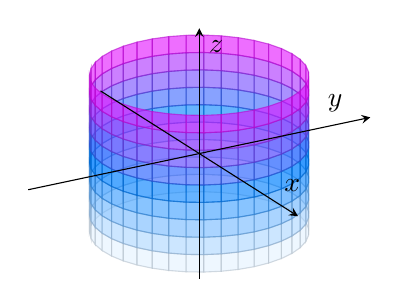
\begin{tikzpicture}
\begin{axis}[
    axis lines=center,
    axis on top,
    xlabel={$x$},
    ylabel={$y$},
    zlabel={$z$},
    xmin=-1.5, xmax=1.5,
    ymin=-1.5, ymax=1.5,
    zmin=-2, zmax=2,
    ticks=none,
    enlargelimits=true,
    view={60}{30}
]
    % Cylinder plot
    \addplot3[
        surf,
        domain=0:360,
        domain y=-1.5:1.5,
        samples=40,
        samples y=10,
        variable=\t,
        variable y=\z,
        colormap/cool,
        opacity=0.6
    ]
    ({cos(t)}, {sin(t)}, {\z});
    
\end{axis}
\end{tikzpicture}
\end{center}
\subsection{Linear Equations across Dimensions}

In $\mathbb{R}^2$, the general form of a linear equation is given by:
\[
Ax + By + C = 0 \quad (A, B, C \in \mathbb{R}, \text{ with } A \text{ and } B \text{ not both zero})
\]
This equation represents a \textit{line} in two-dimensional space.

In $\mathbb{R}^3$, however, the exact same algebraic equation $Ax + By + C = 0$ represents a \textit{plane} parallel to the $z$-axis (since $z$ is a free variable), not a line. 

To uniquely define a line in three-dimensional space, a single linear equation is insufficient; we require a system of \textit{two} independent linear equations (representing the intersection of two non-parallel planes).
